\documentclass[11pt]{article}
% \usepackage{geometry}
% \geometry{margin=0.2in}
% \usepackage[X2]{fontenc}
\usepackage[utf8]{inputenc}
% \usepackage[utf8x]{inputenc}

\nonstopmode
% \usepackage{minted}[cache=false]
\usepackage{graphicx} % Required for including pictures
\usepackage[figurename=Figure]{caption}
\usepackage{float}    % For tables and other floats
\usepackage{amsmath}  % For math
\usepackage{amssymb}  % For more math
\usepackage{fullpage} % Set margins and place page numbers at bottom center
\usepackage{paralist} % paragraph spacing
\usepackage{subfig}   % For subfigures
%\usepackage{physics}  % for simplified dv, and 
\usepackage{enumitem} % useful for itemization
\usepackage{siunitx}  % standardization of si units
\usepackage{hyperref}
% \usepackage{mmacells}
\usepackage{listings}
\usepackage{svg}
\usepackage{xcolor, soul}
\usepackage{bm}
% \usepackage{amsthm}  % For math
\usepackage{mathtools}

% \usepackage{setspace}
% \usepackage{listings}
% \usepackage{listings}
% \usepackage[autoload=true]{jlcode}
% \usepackage{pygmentize}



% \usepackage[margin=1.8cm]{geometry}
\newcommand{\C}{\mathbb C}
\newcommand{\D}{\bm D}
\newcommand{\R}{\mathbb R}
\newcommand{\Q}{\mathbb Q}
\newcommand{\Z}{\mathbb Z}
\newcommand{\N}{\mathbb N}
\newcommand{\PP}{\mathbb P}
\newcommand{\A}{\mathbb A}
\newcommand{\F}{\mathbb F}
\newcommand{\1}{\mathbf 1}
\newcommand{\ip}[1]{\left< #1 \right>}
\newcommand{\abs}[1]{\left| #1 \right|}
\newcommand{\norm}[1]{\left\| #1 \right\|}

\def\Tr{{\rm Tr}}
\def\tr{{\rm tr}}
\def\Var{{\rm Var}}
\def\calA{{\mathcal A}}
\def\calB{{\mathcal B}}
\def\calD{{\mathcal D}}
\def\calE{{\mathcal E}}
\def\calG{{\mathcal G}}
\def\from{{:}}
\def\lspan{{\rm span}}
\def\lrank{{\rm rank}}
\def\bd{{\rm bd}}
\def\acc{{\rm acc}}
\def\cl{{\rm cl}}
\def\sint{{\rm int}}
\def\ext{{\rm ext}}
\def\lnullity{{\rm nullity}}
\DeclareSIUnit\clight{\text{\ensuremath{c}}}
\DeclareSIUnit\fm{\femto\m}
\DeclareSIUnit\hplanck{\text{\ensuremath{h}}}
\usepackage[cache=false]{minted}

% \usepackage{ tipa }

\DeclareUnicodeCharacter{2208}{\ensuremath{\in}}
\DeclareUnicodeCharacter{2082}{\ensuremath{\phantom{}_2}}
\DeclareUnicodeCharacter{03A3}{\ensuremath{\Sigma}}
\DeclareUnicodeCharacter{03C0}{\ensuremath{\pi}}
\DeclareUnicodeCharacter{03C3}{\ensuremath{\sigma}}
\DeclareUnicodeCharacter{03C4}{\ensuremath{\tau}}
\DeclareUnicodeCharacter{0394}{\ensuremath{\Delta}}
\DeclareUnicodeCharacter{2218}{\ensuremath{\circ}}
\DeclareUnicodeCharacter{2A75}{\ensuremath{==}}
\DeclareUnicodeCharacter{03D5}{\ensuremath{\phi}}
\DeclareUnicodeCharacter{2202}{\ensuremath{\partial}}
\DeclareUnicodeCharacter{03C8}{\ensuremath{\psi}}
\DeclareUnicodeCharacter{03C1}{\ensuremath{\rho}}



\definecolor{mintedbackground}{rgb}{0.902, 0.929, 0.906}

\definecolor{cambridgeblue}{rgb}{0.81, 0.9, 0.84}



\sethlcolor{mintedbackground}
\newcommand{\mathcolorbox}[1]{\colorbox{mintedbackground}{$\displaystyle #1$}}

% \lstdefinelanguage{julia}%
%   {morekeywords={abstract,break,case,catch,const,continue,do,else,elseif,%
%       end,export,false,for,function,immutable,import,importall,if,in,%
%       macro,module,otherwise,quote,return,switch,true,try,type,typealias,%
%       using,while},%
%    sensitive=true,%
% %    alsoother={$},%
%    morecomment=[l]\#,%
%    morecomment=[n]{\#=}{=\#},%
%    morestring=[s]{"}{"},%
%    morestring=[m]{'}{'},%
% }[keywords,comments,strings]%

% \lstset{%
%     language         = Julia,
%     basicstyle       = \ttfamily,
%     keywordstyle     = \bfseries\color{blue},
%     stringstyle      = \color{magenta},
%     commentstyle     = \color{ForestGreen},
%     showstringspaces = false,
% }

% $
\usepackage{setspace}

\doublespacing
% \setstretch{1.9}
\begin{document}
{
	\begin{singlespace}
		
\begin{center}
	\hrule
	\vspace{.4cm}
	{\textbf { \large CAS MA 539 --- Methods of Scientific Computing}}
\end{center}
\textbf{Name:}\ Emmy Blumenthal \hspace{\fill} Final Project Report\hspace{\fill}  \textbf{BU ID:} \ U87312711 \\
\textbf{Due Date:}\  Dec 16, 2022   \hspace{\fill} \textbf{Email:}\ emmyb320@bu.edu \ 
\vspace{.4cm}
\hrule
\
% \section*{}

GitHub Repository:  \url{https://github.com/emmyb-bu/ma539-PINNs}

\begin{center}
	\LARGE
	\bf
	Physics-Informed Neural Networks in {\em Julia}: From Scratch and with Packages
\end{center}

\tableofcontents

\end{singlespace}
}
\section{Introduction}

Physics-informed neural networks (PINNs) refer to a set of methods that employ the training of neural networks to approximate solutions to ordinary and partial differential equations.
By choosing the right objective function, a trained neural network can take an independent variable such as position or time and output a dependent variable of interest.
PINNs provide a useful alternative to traditional finite-difference methods because they more easily generalize to new partial differential equations and, with proper care, can address certain stiff equations that might be difficult to solve otherwise.
Remarkably, many problems can be solved quite accurately by using relatively small neural networks, as demonstrated in this project.
PINNs can also solve inverse problems in which one might be interested in estimating some parameter that appears in a partial differential equation given observed data.
In this project, we explore the construction and training of PINNs for several partial differential equations using both the package NeuralPDE.jl and more manual constructions.

\section{PINNs as a Least Squares Problem}

PINNs are trained as a least squares optimization problem.
Generally, a PINN tries to solve a partial differential equation $\mathcal{N}(f(\vec x)) = 0$ for $\vec x \in \Omega$, where $\mathcal{N}$ is some operator that involves derivatives with respect to the variable $\vec x$ and $\Omega$ is the domain over which one is interested in finding a solution, $f(\vec x)$.
Additionally, $f$ must obey some boundary conditions $f(\vec x) = g(\vec x)$ for $\vec x \in \partial \Omega$.
If the solution $f_{\theta}(\vec x)$ is parameterized as a neural network whose weights and biases are a vector of parameters $\theta \in \R^p$ and takes vectors $\vec x \in \Omega$ as inputs, one can calculate the necessary partial derivatives with respect to $\vec x$ using automatic differentiation.
To solve the partial differential equation is then to find some set of parameters $\theta^\star$ so that $\mathcal{N}(f_{\theta^\star} (\vec x)) \approx 0$.
Inspired by the least-squares approach to optimization, we can try to estimate $\theta^\star = \mathrm{argmin}_{\theta} \int_{\Omega}|\mathcal{N}(f_\theta(\vec x))|^2 d\vec x$.
To implement this in practice, we define a set of $N_c$ well-distributed points $\vec \chi_i \in \Omega$ called the {\em collocation points}, a set of $N_b$ well-distributed boundary points $\vec \beta_i \in \partial \Omega$.
The relevant loss function is then the (weighted) sum of mean-squared-errors:
\begin{gather}
	\mathcal{L} ( \{\chi_i\}_{i=1}^{N_c}, \{\beta_i\}_{i=1}^{N_b} ; \theta )=
	\frac{A_c}{N_c} \sum_{i=1}^{N_c} |\mathcal{N}(f_\theta(\chi_i))|^2
	+
	\frac{A_b}{N_b}
	\sum_{i=1} |f_\theta(\beta_i) - g(\beta_i)|^2,
	\\
	\theta^\star = \mathrm{argmin}_{\theta^\star} 
	\mathcal{L} ( \{\chi_i\}_{i=1}^{N_c}, \{\beta_i\}_{i=1}^{N_b};\theta).
\end{gather}
The minimization can be performed in a variety of ways including gradient descent, stochastic gradient descent, or other algorithsm; in this project, we make repeated use of the Broyden–Fletcher–Goldfarb–Shanno (BFGS) algorithm.
For nearly all of these methods, it is necessary to compute gradients of $\mathcal{L} ( \{\chi_i\}_{i=1}^{N_c}, \{\beta_i\}_{i=1}^{N_b};\theta)$ with respect to $\theta$ which is done using automatic differentiation.
Throughout the course of this project, it has proved difficult to efficiently implement calculations of gradients with respect to $\theta$ because computing $\mathcal{N}$ requires taking gradients of $f_\theta(\vec x)$ with respect to $\vec x$.
Another challenge of this minimization is choosing the training weights $A_c, A_b$ so that boundary conditions are well satisfied before the descent algorithm enforces that the solution obeys the partial differential equation; these challenges will be discussed in greater detail in the context of the wave equation.
A similar challenge is choosing the locations of the collocation and boundary points well to emphasize and enforce relevant features; again, this will be discussed in the context of the wave equation.
Like training a neural network for many machine learning applications, performing the necessary minimization requires much manual fine-tuning which can be specific to the relevant partial differential equation and boundary conditions.


\section{The Wave Equation without the NeuralPDE.jl Package}

We solved the wave equation with the following parameters:
\begin{gather}
	\frac{\partial^2 u}{\partial t^2} - \frac{\partial^2 u}{\partial x^2}
	=0
	\\
	u(0,x) = e^{-(t - \tfrac{1}{2})^2/2 \sigma_0^2}, \qquad u(t,0)= u(t,1) = 0, \qquad x \in [0,1], \; t \in [0,1].
\end{gather}
We solved the wave equation with two choices of initial conditions.
For the first trail of solving the wave equation, we chose $\sigma_0 = 0.025$, and used $400$ collocation points distributed as a $20 \times 20$ grid, $80$ boundary points for the $x = 0,1$ boundaries, and $70$ boundary points for the $t = 0$ boundary.
The follow neural network architecture was used:
\begin{singlespace}
\begin{minted}[bgcolor=mintedbackground]{julia}
layerStructure = [
    (2 => 20,NNlib.σ),
    (20 => 20,NNlib.σ),
    (20 => 1,identity)
];
\end{minted}
The structure of the loss function is:
\begin{minted}[bgcolor=mintedbackground,breaklines]{julia}
function waveLoss(model,params)
    DDfs = [FD.jacobian(X -> FD.gradient(Y->model(Y,params)[1],X),Z) for Z in eachcol(collocationPts)];
    return (
        # PDE loss
        NNlib.mean(abs2(DDfs[i][2,2] - DDfs[i][1,1]) for i in 1:nCollocationPts) 
        # Boundary conditions:
        + NNlib.mean(abs2.(ϕmodel(∂xpts,params)[:] - ϕx0)) 
        # ϕ initial value (t=0)
        + 1e2NNlib.mean(abs2.(ϕmodel(∂t0pts,params)[:] - ϕt0))
        # ∂ϕ/∂t initial value (t=0)
        + NNlib.mean(abs2(FD.gradient(Y->model(Y,params)[1],∂t0pts[:,i])[2]-dϕt0[i]) for i in eachindex(dϕt0))
        )
end
\end{minted}
\end{singlespace}
For the initial derivative, we chose $\left.\partial_t u(t,x)\right|_{t = 0} = 0$ and obtained the results pictured below:
\begin{center}
	% \begin{singlespace}
	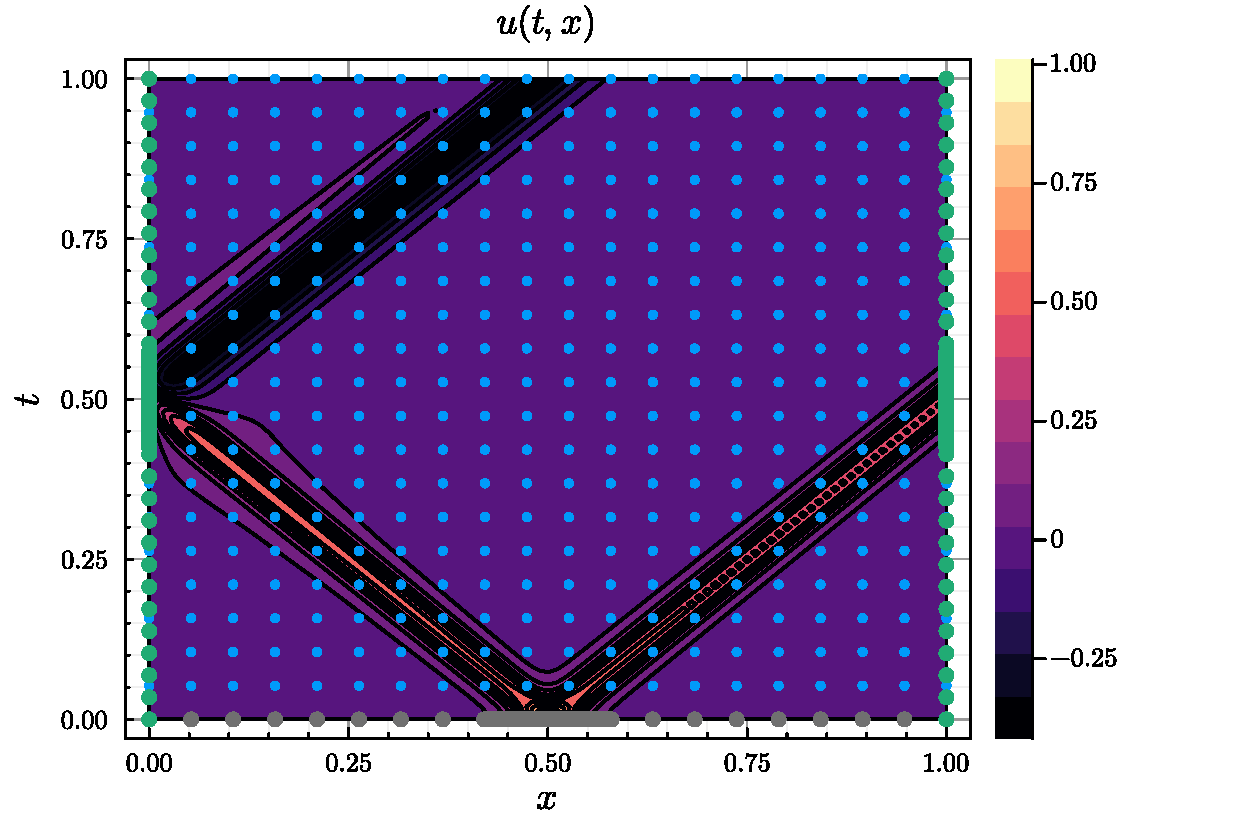
\includegraphics[width=0.9\linewidth]{fig/custom_wave_eq_contour.pdf}
	\\
	Above: Contour plot of solution to wave equation found by training a custom neural network and custom loss function.
	The dots in the center region are the collocation points, the gray dots are the boundary points as $t = 0$, and the green dots are the boundary points at $x = 0,1$.
	Below:
	Plot of solution to the wave equation with respect to the variable $x$ with multiple values of $t$ plotted simultaneously.
	The dots in purple are the boundary points at $t = 0$.
	Evidently, the boundary conditions at $x = 1$ were not properly enforced during the training process because there is no reflection.
	\\
	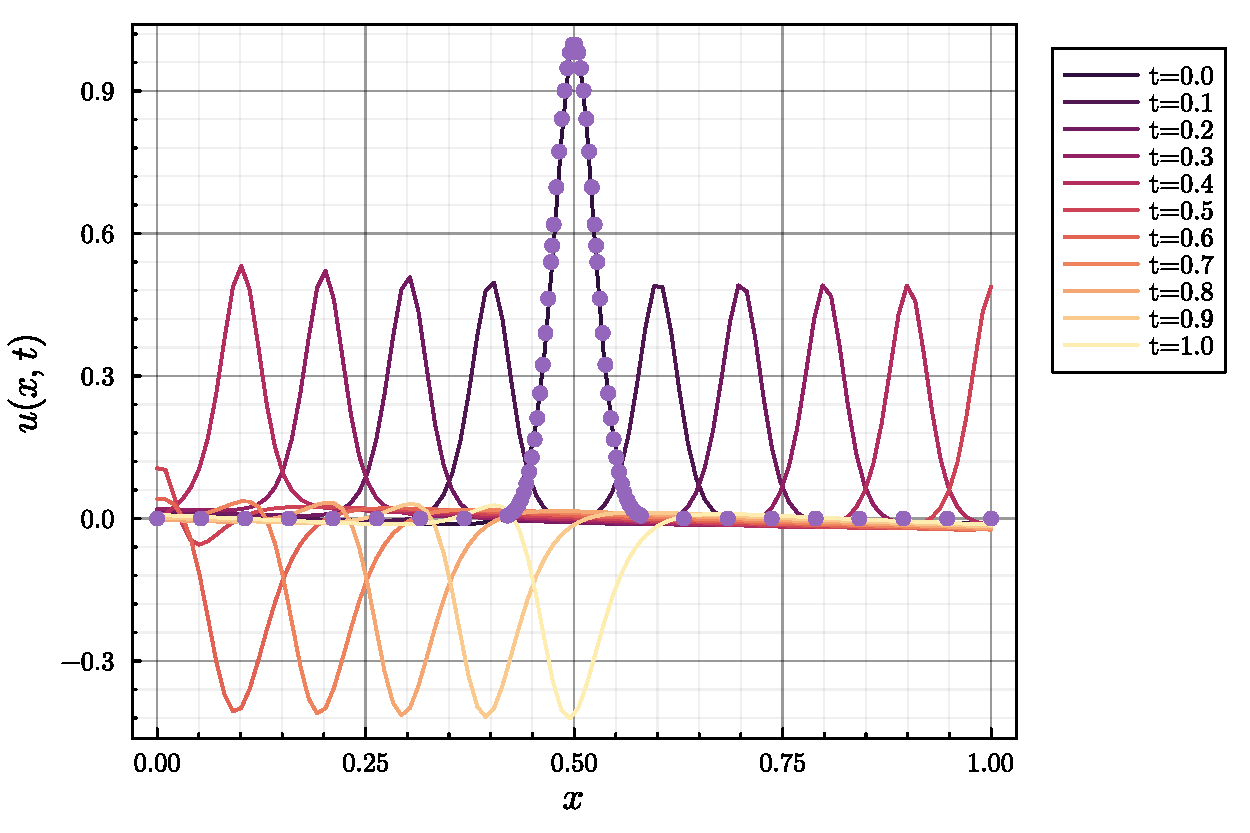
\includegraphics[width=0.9\linewidth]{fig/custom_wave_eq_x.pdf}
% \end{singlespace}
\end{center}
We see that there is no reflection at the boundary $x = 1$ at $t \approx 0.5$ despite what we might expect.
This is a failure in training that we were not able to overcome; it seems that the parameters chosen here may correspond to a local minimum in the loss landscape where the non-zero value of $u$ at the $x = 1$ boundary near $t \approx 0.5$ does not significantly to the loss function.
To attempt to overcome this, we chose a variety of different weights $A_b \gg A_c$ and added additional boundary points near $t \approx 0.5$ to no avail.

This figure also shows that we made the boundary points near $x \sim 0.5$ denser because we want the Gaussian peak of the initial condition to be sampled and fitted properly.
Getting the PINN to express this initial condition was a challenge, but setting $A_b$ to be very large during the early stages of training helped overcome this issue.
It seems that training PINNs even on simpler examples like the wave equation can be a challenge.


% For our next test, we kept the same parameters but now we did not explicitly set a value of $\left.\partial_t u(t,x)\right|_{t = 0}$ to see if training would automatically impose a value.

\section{The Wave Equation with the NeuralPDE.jl Package}

We now compare to our previous result for the wave equation where we used $\left.\partial_t u(t,x) \right|_{t = 0} = 0$ using the NeuralPDE package with the same neural network architecture.
To implement this in NeuralPDE, we had to weight boundary conditions similarly to ensure that they were obeyed.
Luckily, the NeuralPDE interface allows for this using the following option when performing the discretization of the system for training:
\begin{singlespace}	
\begin{minted}[bgcolor=mintedbackground]{julia}
discretization = PhysicsInformedNN(chain, GridTraining([dx,dt]),
	adaptive_loss = NonAdaptiveLoss(pde_loss_weights=1.0,bc_loss_weights=50))
\end{minted}
\end{singlespace}
When doing this, we were able to successfully able to capture the reflection of the wave due to the dirichlet boundary conditions at both $x = 0$ and $x = 1$:
\begin{center}
	% \begin{singlespace}
	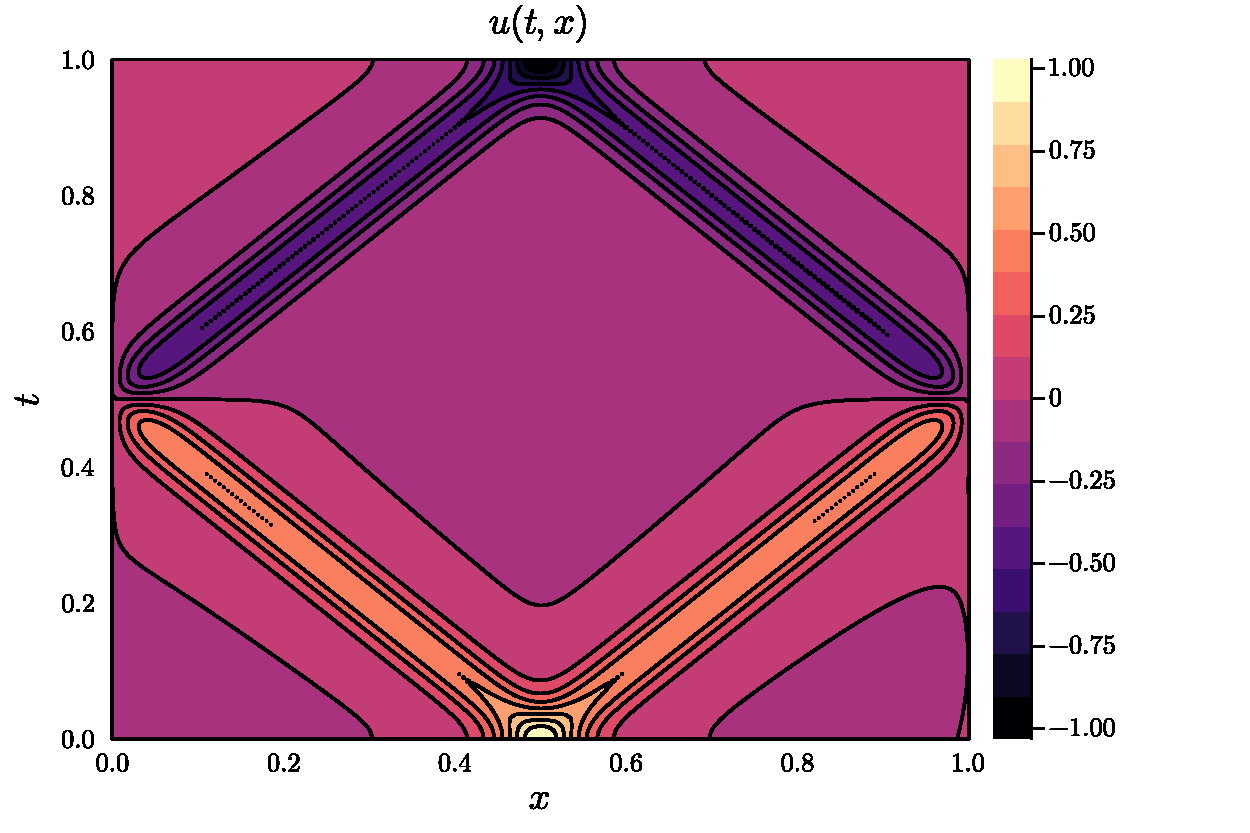
\includegraphics[width=0.9\linewidth]{fig/nice-wave-NeuralPDE.pdf}
	\\
		Above: A contour plot of the solution obtained using the NeuralPDE package.
		In this case, there is reflection off the boundary at $x = 1$ as well as at $x = 0$.
		However, note that $\sigma_0 = 0.04$ where $\sigma_0 = 0.025$ in the implementation without NeuralPDE.
		This may contribute to the presence of the reflection in this version.
		Below: A plot over the variable $x$ at various times $t$.
		Here reflection, the quality of the solution, and the unit wave speed is evident.
	\\
	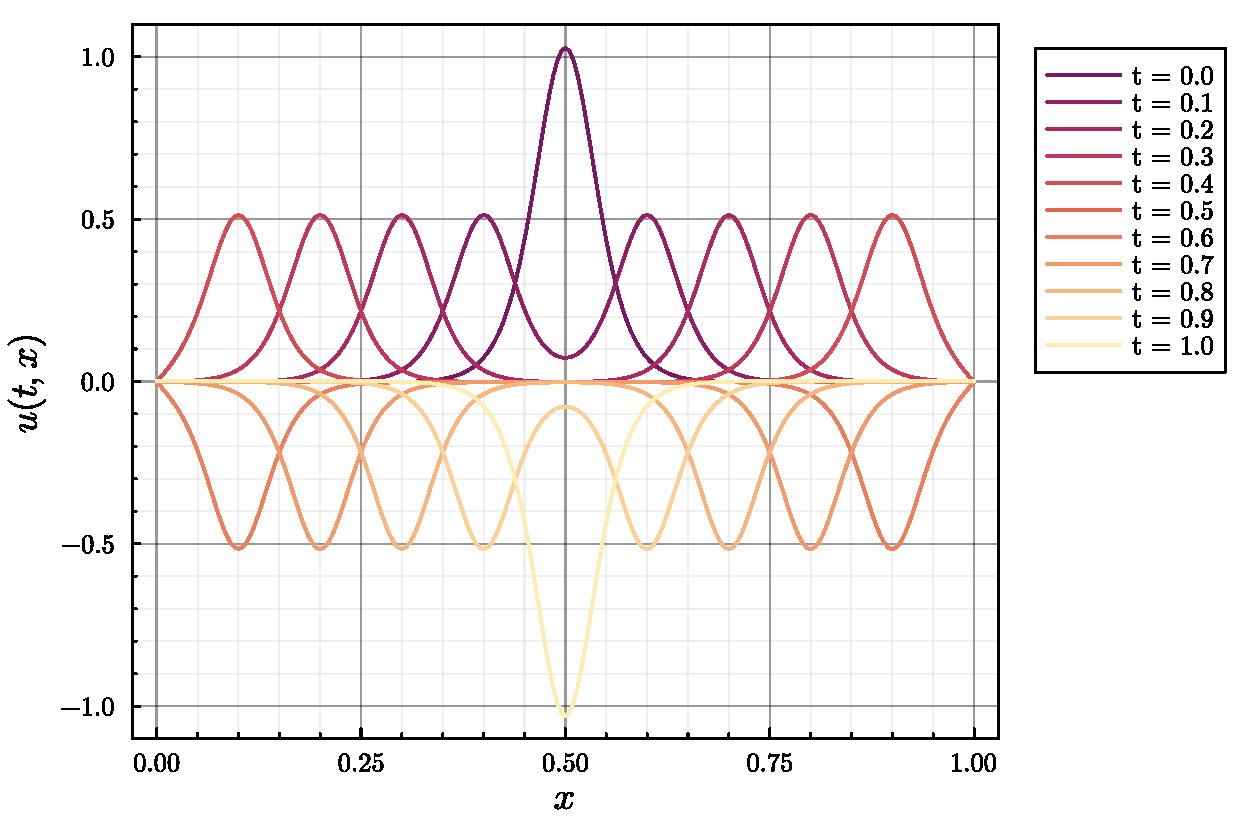
\includegraphics[width=0.9\linewidth]{fig/nice-wave-NeuralPDE-per-t.pdf}
	% \end{singlespace}
\end{center}
Although we were able to successfully capture the reflection, it was still necessary to experiment with initialization, training `strategies' (see \url{https://docs.sciml.ai/NeuralPDE/stable/manual/training_strategies/}), weighting in the loss function, and maximum iterations.
Even for relatively simple partial differential equations and well-constructed libraries, solving partial differential equations using PINNs is a non-trivial task.

An interesting experiment we performed was to not explicitly set a value of $\left.\partial_t u(t,x)\right|_{t = 0}$ to see if training would automatically impose a value.
It turns out that it did; it seemed that training the PINN automatically caused the Gaussian packet to move in the $+x$ direction with unit velocity before reflecting against the boundary at $x = 0$.
Interestingly, after some experimentation and data loss, the movement in the $+x$ direction is not consistent.
It seems that a symmetry is broken when the loss function is optimized without an initial condition.
\begin{center}
	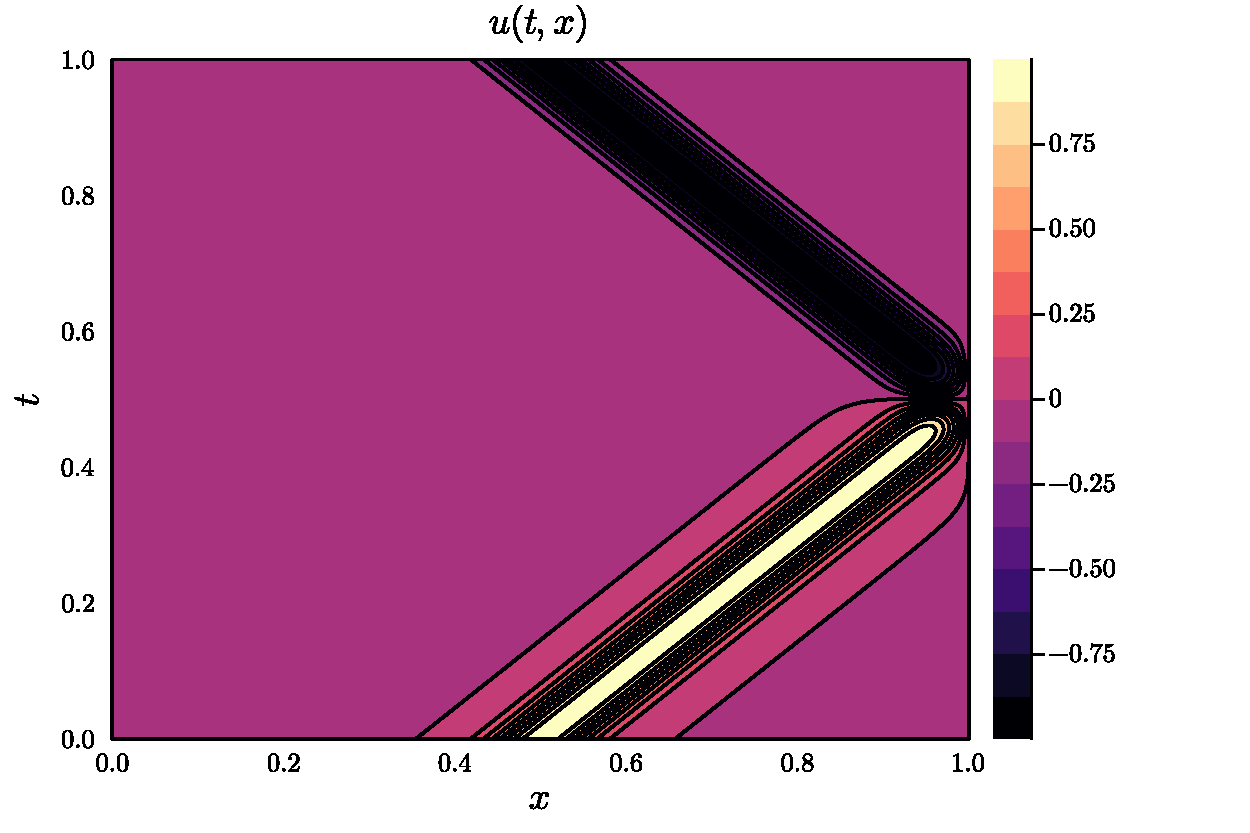
\includegraphics[width=0.9\linewidth]{fig/wave-no-bcs-cont.pdf}
	\\
	Above: Contour plot of the wave equation solved using the NeuralPDE library; no boundary conditions on the initial derivative of the solution are specified, but it seems that in solving, a direction is automatically chosen.
	Below: A plot over the variable $x$ at various times $t$.
	Here we can see the symmetry of the reflection.
	\\
	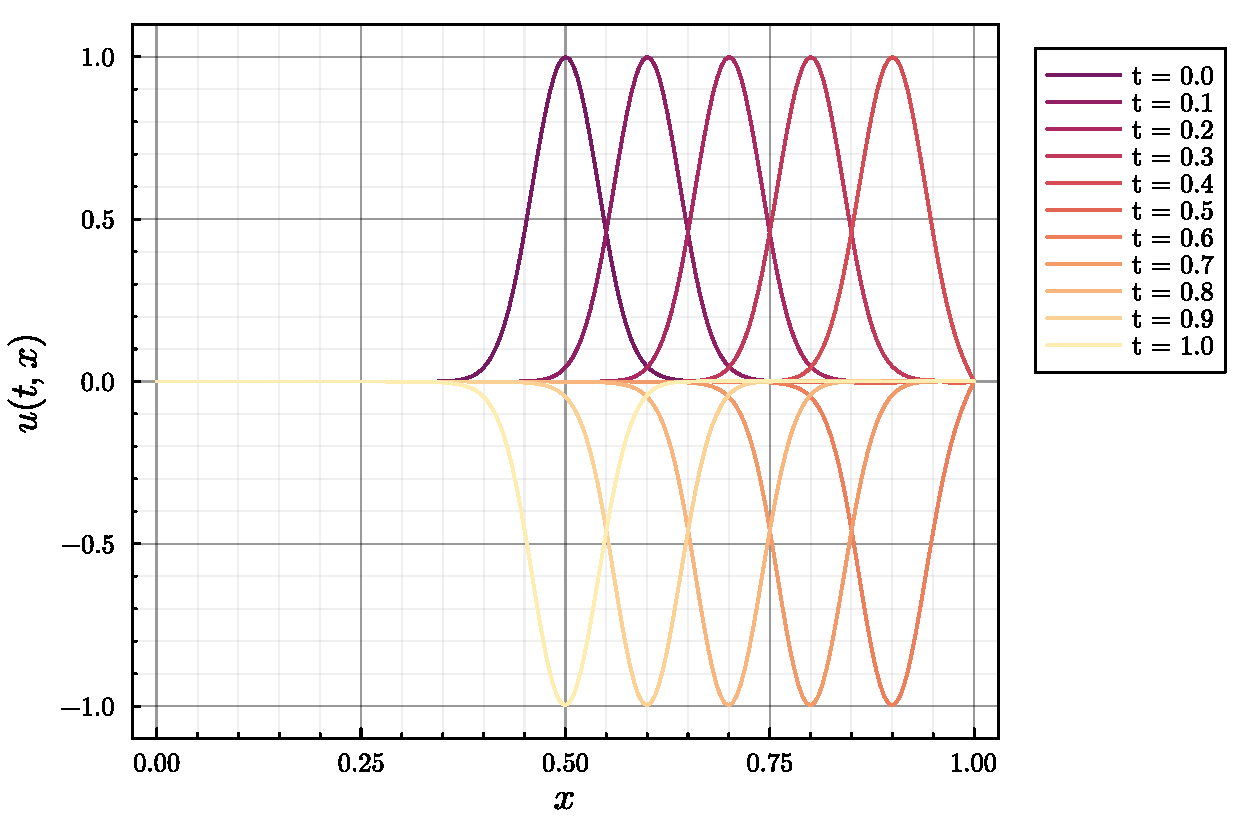
\includegraphics[width=0.9\linewidth]{fig/wave-no-bcs-per-x.pdf}
\end{center}




% \section{The Diffusion Equation without the NeuralPDE.jl Package}




% \section{The Diffusion Equation with the NeuralPDE.jl Package}



% \begin{singlespace}
	\section{Unsuccessful Implementation of the Schro\"odinger Equation with the NeuralPDE.jl Package}
% \end{singlespace}

As part of the various experiments we performed, we attempted to implement the Schr\"odinger equation in the NeuralPDE.jl package with the following set-up:
\begin{singlespace}
\begin{minted}[bgcolor=mintedbackground]{julia}
eqs = [-Dt(ψim(t,x)) ~ -(1/2)*Dxx(ψre(t,x)),
	Dt(ψre(t,x)) ~ -(1/2)*Dxx(ψim(t,x))]

bcs = [ψre(0,x) ~ sin(π*x) + sin(2π*x),
       ψre(t,0) ~ 0.,
       ψim(t,0) ~ 0.,
       ψre(t,1) ~ 0.,
       ψim(t,1) ~ 0.]
\end{minted}
\end{singlespace}
Curiously, when attempting this implementation there were few problems getting the training algorithm to fit the initial/boundary conditions, but it was difficult to observe the behavior of the true solution for times approximately greater than $t = 0.1$.
Curiously, this was also a similar problem when implementing the diffusion equation both with and without the NeuralPDE library.
It seems likely, however, that upon further iterations or access to greater computational resources that training would arrive at a solution.

\section{Challenges Applying PINNs to Higher-Dimensional PDEs}

As part of these explorations, we attempted to implement a PINN solution to the Liouville equation.
This would be an especially useful application because the Liouville equation is often difficult to solve for non-trivial Hamiltonians, and many finite difference methods produce negative values for probability distributions.
By explicitly constructing a neural network that is always non-negative, we can enforce that the solution be non-negative:
\begin{singlespace}
\begin{minted}[bgcolor=mintedbackground]{julia}
eq = Dt(ρ(t,q,p)) ~ Vp(q)*Dp(ρ(t,q,p)) - (p/m)*Dq(ρ(t,q,p));
chain = Lux.Chain(Dense(3,18,Lux.σ),Dense(18,18,Lux.σ),Dense(18,1,X -> X.^2))
\end{minted}
\end{singlespace}
\noindent
While we attempted to train this network, it suffered from the usual problems like not meeting the initial conditions.
Because there are now three variables, each training step took a longer amount of time, so make manual adjustments to the training weights in the loss function was not feasible, so the attempt at solving the Liouville equation was abandoned for this project.

\section{Challenges of Inverse Problems}

Another method that was briefly explored before a loss of data was adding a parameter to the operator.
We briefly experimented by generating analytical data from the wave equation, then training a PINN to infer the wave speed used to generate the data.
This involved an additional term in the least squares loss function which measured the deviation of the PINN solution from the provided generated data.
Preliminary explorations showed some success at inference; it seems that having explicit data to fit to away from the boundary improves the training process.
However, these files were lost and not reproduced.

\section{Further Work and Useful Applications}

There are many open directions to explore given the code written for this project.
It would be interesting to implement this code on several distinct partial differential equations to understand how the nature of an equation influences the training process.
It would be additionally interesting to attempt to apply more powerful computational resources (like graphics processing units) in order to tackle partial differential equations with many independent variables (e.g., the Liouville equation, three-dimensional wave equation).
Revisiting the Schr\"odinger equation would also be interesting because it is implicitly two coupled partial differential equations (the real and imaginary parts of the wave function).
Revisting the Sch\"odinger equation would also provide for an interesting context for exploring the nature of inverse problems.
For example, is it possible to recover parameters that may appear in the potential of a Hamiltonian by minimizing the divergence between the probability density function predicted by the wave function and observations of particle locations?

\section{Viewing Code and Loading Parameters}

All code is on the GitHub repository.
For reproducibility, the trained parameters have been saved and can be loaded in to the relevant scripts for plotting and analysis.
The essential code for this project is in the ./PINNs\_from\_scratch and ./NeuralPDE directories.


\subsection*{A note:}

I did not get as far on this project as I was hoping.
Last week, my computer broke down, and I lost a substantial amount of data including many scripts and saved parameters for this project.
I think I was able to reproduce the essential parts of this project, but I was able to experiment a bit more than is here.

\end{document}





